\section{Hardware}

\FloatBarrier

\subsection{Overview}

\FloatBarrier

\subsection{Controller}
\label{sec_ctrl}
An ESP8266 on a module is selected as microcontroller. The module is used as it already contains the matching network and either an antenna or antenna connector. 
The usage of an ESP32 was considered as well but finally rejected due to the higher cost. 

Three options are considered for the module: ESP-01S, ESP-07S and ESP-12F. \autoref{tab_ESP_modules} lists the modules and their most important specifications. 

\begin{table}[h!]
    \centering
    \begin{zebratabular}{llll}
    \rowcolor{gray} 
        Module  & GPIO  & ADC pin   & Antenna \\
        ESP-01S & 4     & No        & internal \\
        ESP-07S & 11    & No        & external \\
        ESP-12F & 17    & No        & internal \\
    \end{zebratabular}
    \caption[Overview of ESP6288 modules]
            {Overview of ESP6288 modules \cite{AIThinker:ESP_01S} \cite{AIThinker:ESP_07S} \cite{AIThinker:ESP_12F}}
    \label{tab_ESP_modules}
\end{table}

It is possible to solder any of the modules that is listed in \autoref{tab_ESP_modules} on the PCB. The ESP-07S can be soldered on the same footprint as the ESP-12F. The ESP-01S footprint could be fitted inside the ESP-12F footprint. Special car must be taken in that case, as the ESP-07S has an exposed pad. Only the GND pin of the ESP-01S is allowed to touch the area of the exposed pad to prevent short-circuits when the ESP-07S is mounted. \cite{AIThinker:ESP_07S}\cite{AIThinker:ESP_12F}

The ESP module is powered directly from the \qty{3.3}{\volt} supply. The design of the \qty{3.3}{\volt} supply is documented in \secref{sec_power_3V3}. 

The EN pin and the RST pin are pulled to \qty{3.3}{\volt} with a pull-up resistor each. The GPIO pinout is listed in \autoref{tab_ESP_pinout}. 

\begin{table}[h!]
    \centering
    \begin{zebratabular}{lllll}
        \rowcolor{gray} 
        Signal      & ESP-01S   & ESP-07S   & ESP-12F   & Description \\
        DATA        & GPIO0     & GPIO15    & GPIO15    & LED data \\
        KILL        & GPIO2     & GPIO13    & GPIO13    & Turn-off command \\
        HALL        & N/A       & GPIO14    & GPIO14    & Presence detection from hall sensor \\
        VBAT\_MON   & N/A       & ADC       & ADC       & Battery voltage monitor \\
    \end{zebratabular}
    \caption{ESP module pinout}
    \label{tab_ESP_pinout}
\end{table}

\FloatBarrier

\subsection{LED}
\label{sec_LED}
Addressable NeoPixel acp{LED} of the type WS2813 from WorldSemi are used to illuminate the cone. Four \acp{LED} are evenly distributed on the top side of the PCB to illuminate the enclosure of the NightCone. A total of 16 \acp{LED} are aligned in the shape of a circle on the bottom side. The purpose of those \acp{LED} is the illumination of the ground around the cone and the cone from above. 

Each NeoPixel \ac{LED} contains a controller and three single \acp{LED} in the colors red, green and blue. The brightness of each LED can be set through an interface. On the interface a bit is represented by a pulse. The value of the bit is encoded in the pulse length. A reset command is sent by pulling the data line low for an certain time $t_{reset}$. \autoref{fig_neopixel_bit} shows the signal shape of 0s, 1s and the reset pulse. The specific timing depends on the LED type and is listed in \autoref{tab_neopixel_timing}. \cite{Worldsemi:WS2813B-B}\cite{Worldsemi:WS2813B-V5}\cite{Worldsemi:WS2813C}\cite{Worldsemi:WS2813E}

\begin{figure}[h!]
    \centering
    \begin{tikztimingtable}
        0s    & 0.2L25{0.6H1.4L}0.2H\\
        1s    & 0.2L25{1.4H0.6L}0.2H\\
        Reset & 0.2H50L0.2H\\
    \end{tikztimingtable}
    \caption[NeoPixel bits, timing not representative]
            {NeoPixel bits, timing not representative, see \autoref{tab_neopixel_timing} for exact timing}
    \label{fig_neopixel_bit}
\end{figure}

\begin{table}[h!]
    \centering
    \begin{zebratabular}{lllllll}
        \rowcolor{gray}
        LED type    & $t_{0_H}$ [\si{\nano\second}] & $t_{0_L}$ [\si{\nano\second}] & $t_{1_H}$ [\si{\nano\second}] & $t_{1_L}$ [\si{\nano\second}] & $t_{Reset}$ [\si{\micro\second}]  & Pin 1 \\
        WS2813B-B   & 220 \ldots 380                & 580 \ldots 1600               & 580 \ldots 1600               & 220 \ldots 420                & > 280                             & VCC   \\
        WS2813B-V5  & 220 \ldots 380                & 580 \ldots 1000               & 580 \ldots 1600               & 580 \ldots 1000               & > 280                             & BO    \\
        WS2813C     & 220 \ldots 380                & 580 \ldots 1600               & 580 \ldots 1600               & 220 \ldots 420                & > 280                             & VCC   \\
        WS2813E     & 220 \ldots 380                & 580 \ldots 1600               & 580 \ldots 1600               & 220 \ldots 420                & > 280                             & NC    \\
    \end{zebratabular}
    \caption[LED timing overview]
            {LED timing overview \cite{Worldsemi:WS2813B-B}\cite{Worldsemi:WS2813B-V5}\cite{Worldsemi:WS2813C}\cite{Worldsemi:WS2813E}}
    \label{tab_neopixel_timing}
\end{table}

Each \ac{LED} has an internal buffered shift-register with a length of \qty{24}{\bit}. Every bit that is received shifts the content of the register for \todo{better word (um)} one bit. The last bit that is shifted out of the register is transmitted to the successive \ac{LED} in the chain. When a reset signal is received, the content of the shift-register is loaded into the buffer and the brightness of the three colored \acp{LED} is updated. The register definition is shown in \autoref{tab_neopixel_register}. \cite{Worldsemi:WS2813B-B}\cite{Worldsemi:WS2813B-V5}\cite{Worldsemi:WS2813C}\cite{Worldsemi:WS2813E}

\begin{table}[h!]
    \centering
    \begin{tabular}{|l|l|l|l|l|l|l|l|l|}
        \hline
        Bit     & 1  & 2  & 3  & 4  & 5  & 6  & 7  & 8  \\
        \hline
        Data    & G7 & G6 & G5 & G4 & G3 & G2 & G1 & G0 \\
        \hline
        \hline
        Bit     & 9  & 10 & 11 & 12 & 13 & 14 & 15 & 16 \\
        \hline
        Data    & R7 & R6 & R5 & R4 & R3 & R2 & R1 & R0 \\
        \hline
        \hline
        Bit     & 17 & 18 & 19 & 20 & 21 & 22 & 23 & 24 \\
        \hline
        Data    & B7 & B6 & B5 & B4 & B3 & B2 & B1 & B0 \\ 
        \hline
    \end{tabular}
    \caption{NeoPixel register definition}
    \label{tab_neopixel_register}
\end{table}

The advantage of the WS2813 type over the widely used WS2812 is the additional backup input. The input of each \ac{LED} is also connected to the backup input of the next \ac{LED} in the chain. This allows the chain to continue operation even when a \ac{LED} has failed completely. The chain continues to operate with up to half of the \acp{LED} failed, as long as there are no successive failed \acp{LED}. On some \ac{LED} types a separate backup output exists on pin 1. Refer to \autoref{tab_neopixel_timing} for this information. 

\subsection{Failsafe}
\label{sec_failsafe}
\ReqRef{R:Failsafe} requires the \acp{LED} to illuminate in a controlled way after a controller failure. The simplest way to control the \acp{LED} is to send 1's followed by a reset pulse. This causes the \acp{LED} to light up white with the highest intensity. To ensure that all \acp{LED} turn on, the number of bits sent must be at least the number of bits per \ac{LED} multiplied by the number of \acp{LED}. A missing-pulse detector with an edge detector is used to detect a controller failure. Depending on the state of this detector, the signal from the controller or the failsafe signal is selected for the \acp{LED}. 

The controller is powered with a voltage of \qty{3.3}{\volt}, which results in the same level for the output signals. The \acp{LED} are powered by the \qty{5.2}{\volt} supply and therefore expect an input signal with a similar voltage. A level-shifter converts the signal from \qty{3.3}{\volt} to \qty{5.2}{\volt} and also inverts the signal. An edge-detector avoids that a static signal triggers the missing-pulse detector. The inverter of the edge-detector is used to recondition the input signal and invert it again. The edge-detector generates a low pulse when a rising edge is detected. \autoref{fig_failsafe_edge}

\begin{figure}[h!]
    \centering
    \includegraphics[page=3, scale=\schscale, trim=25 475 738 165, clip]{\schfile}
    \caption{Levelshifter and edge detector}
    \label{fig_failsafe_edge}
\end{figure}

The missing-pulse detector is built with a XL555, which is a pin-compatible \ac{CMOS} derivate of the NE555 timer. \todo{reference to XL555 datasheet} The timing capacitor C10 is continuously charged by R13. The low pulse from the edge-detector discharges the capacitor through D10 and R20. R20 limits the current to protect the output of the edge-detector. In case D10 is not able to discharge C10 quick enough, Q4 can be added to increase the discharge current. The output of the edge-detector is also connected to the TRIG input of the timer and sets the internal flipflop when a pulse is detected. When the capacitor voltage reaches the CONT voltage, which is $\frac{2}{3}$ of the supply voltage, the flipflop of the timer is reset, which is interpreted as controller-failure. \autoref{fig_failsafe_missing_pulse}

\begin{figure}[h!]
    \centering
    \includegraphics[page=3, scale=\schscale, trim=360 420 510 165, clip]{\schfile}
    \caption{Missing-pulse detector}
    \label{fig_failsafe_missing_pulse}
\end{figure}

An astable multivibrator with a XL555 generates the pulse pattern for a series of 1s. The timing requirements depends on the \ac{LED} type. \autoref{tab_neopixel_timing} shows the timing requirements for each \ac{LED} type that can be used. The formula for the timing as astable multivibrator is inaccurate in the frequency range that is used to generate the data pulse. \todo{Reference to XL555 datasheet} Therefore the component values for the oscillator were iterated on a test circuit using a TLC555 which is very similar to the XL555 that is used. The resulting values are listed in \autoref{tab_failsafe_bit_values}. The bit signal is fed into a ripple counter to count the number of bits and generate the reset pulse. \todo{Number of stages in the reset counter} \autoref{fig_failsafe_bit_counter}

\begin{table}[h!]
    \centering
    \begin{zebratabular}{llllll}
        \rowcolor{gray}
        LED &
        $t_{1_H}$ &
        $t_{1_L}$ &
        R17 &
        R19 &
        C11 \\
        B-B, C, E &
        \qty{1.09}{\micro\second} &
        \qty{320}{\nano\second} &
        \qty{1.5}{\kilo\ohm}   &
        \qty{270}{\ohm}        &
        \qty{470}{\nano\farad} \\
        B-V5 &
        \qty{1.09}{\micro\second} &
        \qty{790}{\nano\second} &
        \qty{910}{\ohm} &
        \qty{1.2}{\kilo\ohm} &
        \qty{470}{\nano\farad} \\
    \end{zebratabular}
    \caption{Component values for the astable multivibrator, obtained from TLC555 test circuit iteration}
    \label{tab_failsafe_bit_values}
\end{table}

\begin{figure}[h!]
    \centering
    \includegraphics[page=3, scale=\schscale, trim=275 255 370 330, clip]{\schfile}
    \caption{Bit-pulse generator with counter for reset generation}
    \label{fig_failsafe_bit_counter}
\end{figure}

The data pulse and the reset signal are combined to the failsafe signal with an AND gate. A multiplexer (74LVC1G157) selects either the signal from the controller or the failsafe signal to send to the \acp{LED} based on the state of the missing-pulse detector. 

\begin{figure}[h!]
    \centering
    \includegraphics[page=3, scale=\schscale, trim=700 380 100 350, clip]{\schfile}
    \caption{Signal selector}
    \label{fig_failsafe_mux}
\end{figure}

\FloatBarrier

\subsection{Battery}
\label{battery}
The NightCone is powered by a single \ac{LiIon} battery cell. The cell is mounted in the center of the NightCone. 

To design the required battery capacity, the energy consumption of each component is calculated. The efficiency $\eta_{5V2}$ and $\eta_{3V3}$ of each voltage converter is assumed to be 0.9. 

The average current consumption of the ESP module is \qty{71}{\milli\ampere} at a supply voltage of \qty{3.3}{\volt}. \cite{AIThinker:ESP_12F}
\begin{align}
    P_{ESP} = \dfrac{V_{ESP} \cdot I_{ESP}}{\eta_{5V2} \cdot \eta_{3V3}} = \dfrac{\qty{3.3}{\volt} \cdot \qty{71}{\milli\ampere}}{0.9 \cdot 0.9} = \qty{289.3}{\milli\watt}
\end{align}

The current of a single \ac{LED} is up to \qty{16}{\milli\ampere} for all three colors. \cite{Worldsemi:WS2813E}
\begin{align}
    P_{LED} = \dfrac{V_{LED} \cdot I_{LED} \cdot 3 \cdot n_{LED}}{\eta_{5V2}} = \dfrac{\qty{5.2}{\volt} \cdot \qty{16}{\milli\ampere} \cdot 3 \cdot 20}{0.9} = \qty{5.547}{\watt}
\end{align}

As the current consumption of the failsafe circuit is assumed to be much smaller than that of the \acp{LED} it is neglected for the energy estimation. 

The minimum oparation time is defined in \ReqRef{R:Time}. 
\begin{align}
    W = \left(P_{ESP} + P_{LED}\right) \cdot t = \left(\qty{289.3}{\milli\watt} + \qty{5.547}{\watt}\right) \cdot \qty{4}{\hour} = \qty{23.35}{\watt\hour}
\end{align}
\begin{align}
    Q = \dfrac{W}{V_{nom}} = \dfrac{\qty{23.35}{\watt\hour}}{\qty{3.6}{\volt}} = \qty{6.31}{\ampere\hour}
\end{align}

A capacity of \qty{6.31}{\ampere\hour} would require a 26650 cell. As the cone is not expected to be set to the maximum brightness for all three colors, a capacity of about \qty{5}{\ampere\hour} is expected to be sufficient. This allows the use of a 21700 cell, which reduces the cost of the battery solution. A 18650 cell could also fit in the enclosure, but would only be available with a capacity of \qty{3}{\ampere\hour}, which is assumed to be insufficient. 

The cell is mounted in the center of the NightCone. The \ac{PCB} includes an opening in the center for the cell to fit through. Nickel strips are spotwelded to the cell. The strips are soldered to solder pads to connect the battery to the electronics. The positive lead is connected soldered to the top side of the \ac{PCB}, the negative lead to the bottom side. 

\subsection{Battery Management System}
\label{sec_bms}
The battery management system is pretty simple using a two IC solution. The used DW01A \cite{Puolop:DW01A} is a low cost \ac{LiIon} protection IC. It protects the battery from the following issues: 
\begin{itemize}
	\item Overvoltage at $\qty{4.3(0.05)}{\V}$  after $\qtyrange{110}{200}{\ms}$
	\item Undervoltage at $\qty{2.50(0.10)}{\V}$after $\qtyrange{55}{200}{\ms}$
	\item Overcurrent
\end{itemize}
This covers requirement \ReqRef{R:Current} and partially \ReqRef{R:BMS}. The overtemperature protection is done in the charger and therefore only available during charging. 

The overcurrent protection is realized using the voltage drop over the two AO3400A \cite{AOSMD:AO3400A}. The DW01A IC features two types of over current protection. 

The fast over current protection triggers at nominal $\qty{1.36}{\V}$ with a blanking time of $\qtyrange{400}{600}{\ms}$. This leads to the following thresholds: 
\begin{align}
	I_\mathrm{SC;fast,min} &= \frac{V_\mathrm{SC,fast,min}}{2\cdot R_\mathrm{AO3400A,max}}=\frac{\qty{0.82}{\V}}{2\cdot\qty{48}{\milli\ohm}}=\qty{8.5}{\A}\\
		I_\mathrm{SC;fast,typ} &= \frac{V_\mathrm{SC,fast,typ}}{2\cdot R_\mathrm{AO3400A,typ}}=\frac{\qty{1.36}{\V}}{2\cdot\qty{24}{\milli\ohm}}=\qty{28.3}{\A}\\
		I_\mathrm{SC;fast,max} &= \frac{V_\mathrm{SC,fast,max}}{2\cdot R_\mathrm{AO3400A,typ}}=\frac{\qty{1.75}{\V}}{2\cdot\qty{24}{\milli\ohm}}=\qty{36.5}{\A}\\
\end{align}


\begin{figure}[h!]
    \centering
    \includegraphics[page=25, scale=\schscale, trim=720 230 75 420, clip]{\schfile}
    \caption{Battery management system}
    \label{fig_bms}
\end{figure}

The slow over current protection triggers at nominal $\qty{150(20)}{\milli\V}$ after a blanking time of $\qtyrange{7}{20}{\ms}$. This leads to the following values: 
\begin{align}
	I_\mathrm{SC;slow,min} &= \frac{V_\mathrm{SC,slow,min}}{2\cdot R_\mathrm{AO3400A,max}}=\frac{\qty{130}{\milli\V}}{2\cdot\qty{48}{\milli\ohm}}=\qty{1.4}{\A}\\
		I_\mathrm{SC;slow,typ} &= \frac{V_\mathrm{SC,slow,typ}}{2\cdot R_\mathrm{AO3400A,typ}}=\frac{\qty{150}{\milli\V}}{2\cdot\qty{24}{\milli\ohm}}=\qty{3.1}{\A}\\
		I_\mathrm{SC;slow,max} &= \frac{V_\mathrm{SC,slow,max}}{2\cdot R_\mathrm{AO3400A,typ}}=\frac{\qty{170}{\milli\V}}{2\cdot\qty{24}{\milli\ohm}}=\qty{3.5}{\A}\\
\end{align}

If the maximum current is $I_\mathrm{max}=\frac{P_\mathrm{ESP}+P_\mathrm{LED}}{V_\mathrm{bat,min}}=\frac{\qty{289.3}{\milli\W} + \qty{5.547}{\W}}{\qty{2.5}{\V}}=\qty{2.33}{\A}$, the current threshold is exceeded, if the resistance of both MOSFETS is at the maximum value. This must be extensively tested. 

The resettable fuse acts as a last resort, if the DW01A is malfunctioning.

\FloatBarrier

\subsection{Charger}
\label{sec_charger}

The cone can be charge by using three screws as connectors on the outside to fulfil \ReqRef{R:Charging}. Two of the three circumferentially distributed screws must be connected to a voltage of $\qtyrange{5.25}{6.5}{\V}$, as it can be seen in Figure \ref{fig_chg_connection}. 
\begin{figure}[h!]
	\centering
	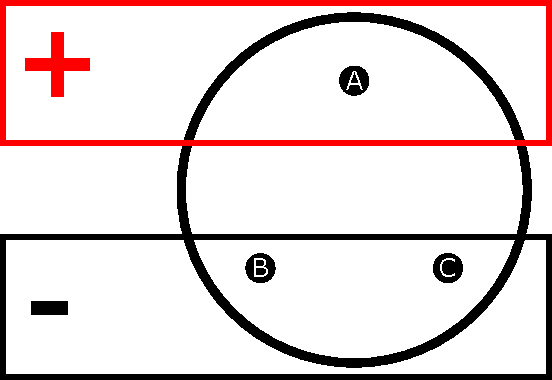
\includegraphics[scale=0.5]{img/CAD_Charging.pdf}
	\caption{Charging pin connection}
	\label{fig_chg_connection}
\end{figure}
The $\qty{1.5}{\A}$ fuse protects the charging circuit. The six shottky rectifier diodes allow to use any pin for positive and negative supply. The two $\qty{1}{\ohm}$ resistors are used to reduce the required voltage drop inside the charging IC and to act as linear impedance for the $\qty{6.8}{\V}$ transient voltage suppression diode. The diode has a reverse stand-off voltage of $\qty{5.8}{\V}$ and a minimum breakdown voltage of $\qty{6.45}{\V}$. 
This allows a maximum input voltage of 
\begin{align}
	V_\mathrm{in,max} &= V_\mathrm{R,TVS} + 2\cdot V_\mathrm{f,SS34} = \qty{5.8}{\V}+ 2\cdot \qty{0.35}{\V}=\qty{6.5}{\V}\\
	V_\mathrm{in,min,end} &= V_\mathrm{bat,max} + V_{drop, TP4056} + 2\cdot V_{f,SS34} = \qty{4.2}{\V} + \qty{0.03}{\V} + 2\cdot \qty{0.35}{\V} = \qty{4.93}{\V}
\end{align}
The voltage drop on the voltage reduction resistor can be neglected for the first two cases because the maximum voltage must be followed also for the final charge phase, where the current converges to zero and the same is the case for the minimal voltage when finishing charging. 
The voltage drop is considered in the following case for the minimum voltage at full charging current at the highest voltage:
\begin{align}
	V_\mathrm{in,min,charge} &= V_\mathrm{bat,charge} + V_\mathrm{drop, TP4056} + 2\cdot V_\mathrm{f,SS34} + R \cdot I_\mathrm{chg}\\
	&= \qty{4.1}{\V} + \qty{0.03}{\V} + 2\cdot \qty{0.35}{\V} + \qty{0.5}{\ohm} \cdot  \qty{0.78}{\A} = \qty{5.22}{\V}
\end{align}

\begin{figure}[h!]
    \centering
    \includegraphics[page=25, scale=\schscale, trim=60 485 685 135, clip]{\schfile}
    \caption{Charging rectifier and input protection}
    \label{fig_chg_input}
\end{figure}

The charging IC TP4056 \cite{MSKSEMI:TP4056} monitors the cell temperature during the charging process by evaluating the voltage drop of the used $\qty{10}{\kilo\ohm}$ \ac{NTC}. This covers the missing part of \ReqRef{R:BMS}. The voltage at the Temp pin is evaluated as ratio to the supply voltage. The operative range is $\num{0.45} \cdot \mathrm{VCC}$ to $\num{0.8} \cdot \mathrm{VCC}$. The resistor divider is designed to operate in a temperature range from $\qtyrange{5}{50}{\celsius}$. The resistors $R_5$ and $R_7$ are derived using these formulas: 
\begin{align}
R_7 &= \frac{R_\mathrm{th,low}\cdot R_\mathrm{th,high}}{(V_\mathrm{th,low}-1)\cdot R_\mathrm{th,high} + \left(\frac{V_\mathrm{th,low}}{V_\mathrm{th,high}}-V_\mathrm{th,low}\right)\cdot R_\mathrm{th,low}}\\
R_5 &= R_7\cdot R_\mathrm{th,low}\cdot \frac{1-V_\mathrm{th,high}}{V_\mathrm{th,high}\cdot (R_7+R_\mathrm{th,low})}
\end{align}
The resulting values where then adapted to use resistors already used in other parts of the schematic, which also matched quite well. 

\begin{figure}[h!]
    \centering
    \includegraphics[page=25, scale=\schscale, trim=420 435 110 120, clip]{\schfile}
    \caption{Charger}
    \label{fig_charger}
\end{figure}

The charging current is set to $\qty{780}{\mA}$ by using the $\qty{1.5}{\kilo\ohm}$ resistor. The charger has a trickle current feature that charges the battery with a low current of $\qty{130}{\milli\A}$ if the battery voltage is below $\qty{2.9}{\V}$. \\
In the schematic, both \acp{LED} are marked as green. \ac{LED} D6 is replaced by a red \ac{LED}. The functions of the \acp{LED} are summarized in the following table

\begin{table}[h!]
    \centering
    \begin{zebratabular}{lll}
        \rowcolor{gray}
        Charging State &
        LED Green &
        LED Red \\
        Charging & off & on \\
        Charging terminated & on & off\\
        Temp error, no power or battery & off &off\\
        No battery & on & flashing ($\qtyrange{1}{4}{\s}$)
    \end{zebratabular}
    \caption{Charger LED Signals}
    \label{tab_chg_led}
\end{table}

\FloatBarrier

\subsection{On/off controller}
\label{sec_onoff}

As \ReqRef{R:Rain} requires the cone to be able to operate in rain , it must be possible to turn the NightCone on and off without opening it. To fulfill this requirement, one method to enable the NightCone and two methods to disable it are implemented. The hall sensor U30 (UHE4913) detects the presence of a magnet. When a magnet is detected, the output of the sensor is pulled low. This pulls the enable input of the boost converter U28 towards the battery voltage, which enables the converter. As the hall sensor is directly connected to the battery and therefore always powered, a sensor with a low operating current must be chosen. The selected boost converter (TPS61023) completely disconnects the output from the input when the converter is disabled. This is necessary because the output voltage of a boost converter is always at least slightly lower than the input voltage due to the body diode of the highside \ac{MOSFET}. \cite{TI:TPS61023}. \todo{Check link to TPS61023 datasheet}

The controller can send a KILL signal to the on/off controller. To ensure, that a static high signal is not able to shut down the NightCone, the signal is AC coupled and rectified. To disable the NightCone, a series of pulses must be sent to the KILL signal which charges the capacitor C71. When the threshold voltage of Q10 is reached, the \qty{5.2}{\volt} converter is disables by pulling the EN signal low. 

The requirement \ReqRef{R:Disable} demands an analog shutdown device. This is implemented by supervising the voltage on the charging input. When a voltage is detected, Q9 pulls the EN signal to GND, which disables the \qty{5.2}{\volt} converter. The threshold level can be adjusted by changing the voltage divider R94 and R96. This ensures that the NightCone is automatically disabled when it is connected to the charging station. 

During development and debugging it is advantageous to allow the operation of the NightCone while the battery is being charged. To allow this operation mode, the signal of the hall sensor is prioritized over both turn off signals. This means, that the NightCone can not be turned off when the presence of a magnet is detected. For the schematic of the on/off controller, see \autoref{fig_onoff}. 

\begin{figure}[h!]
    \centering
    \includegraphics[page=26, scale=\schscale, trim=30 80 550 245, clip]{\schfile}
    \caption{On/off controller}
    \label{fig_onoff}
\end{figure}

\FloatBarrier

\subsection{Converter \qty{5.2}{\volt}}
\label{sec_power_5V2}

\begin{figure}[h!]
    \centering
    \includegraphics[page=26, scale=\schscale, trim=280 395 435 245, clip]{\schfile}
    \caption{\qty{5.2}{\volt} converter}
    \label{fig_power_5V2}
\end{figure}

\FloatBarrier

\subsection{Converter \qty{3.3}{\volt}}
\label{sec_power_3V3}

\begin{figure}[h!]
    \centering
    \includegraphics[page=26, scale=\schscale, trim=660 395 25 265, clip]{\schfile}
    \caption{\qty{3.3}{\volt} converter}
    \label{fig_power_3V3}
\end{figure}

\FloatBarrier

\subsection{Modifications from index AA to index AB}

\subsubsection{Feedforward capacitor in \qty{5.2}{\volt} and \qty{3.3}{\volt} supply}
The feedforward capacitors in the feedback networkof the two converters are not meant to be mounted. It must either be removed or a value must be selected to ensure loop stability. 

\subsubsection{Charging LED color}
To reduce the cost of the first prototypes, the color of the charging \ac{LED} was changed to green. For correct operation, it needs to be changed to red. 

\subsection{Modifications from index AA to index BA}

\subsubsection{Programming connector}
A Tag-Connect interface (TC2030) should be added for programming the ESP module. If there is enough space, the footprint with legs should be used. Necessary signals are TX, RX, RESET and GIPO0. 

\subsubsection{ESP-01S}
The GPIO count of the ESP-01S is insufficient for the complete functionaility and it lacks an \ac{ADC} input. The option to mount it can therefore be removed. 

\subsubsection{Memory for configuration data}
To reduce the number of write cycles on the flash memory of the ESP8266, an additional nonvolatile memory should be added to store configuration data. It needs to be able to endure frequent write operation. From a first analysis, an \ac{I2C} \ac{EEPROM} would be ideal. 

\subsubsection{GPIO}
Due to the addition of an \ac{I2C} \ac{EEPROM}, the \ac{GPIO} pins need to be rearranged, as on index A, the signal from the hall sensor is connected to GPIO14, which is used as SCL. 

\subsubsection{HW ID}
A hardware ID should be implemented to indicate different hardware revisions to the software. This can be implemented by connecting GPIO pins or by changing the I2C address of the EEPROM. No additional HW should be implemented for the HW ID. 

\subsection{Over-current protection}
The over-current protection on the prototype triggers below the maximum current, because the maximum resistance of the used MOSFETs is to high. The typical value would be sufficient. The fuse $(\qty{1.5}{\A}$ is as well too low. 

\subsubsection{Failsafe counter output}
The failsafe counter only counts to 256. With a total of 20 \acp{LED}, 480 pulses are required to turn on all \acp{LED}. Therefore FS\_RESET must be connected to Q9 instead of Q8. 

\subsubsection{Quiescent current}
D11 causes about \qty{40}{\micro\ampere} of quiescent current (up to \qty{500}{\micro\ampere} according to datasheet) and is unnecessary as the body diode of Q5 is parallel. D11 can be removed. 

\subsubsection{Power indication LED}
The power indication \acp{LED} are unnecessary and can be removed or set to NB. 

\subsubsection{GPIO 15 for FW upload}
GPIO 15 must always be pulled low for Flash boot and FW upload. R16 must be replaced by a $\qty{10}{\kilo\ohm}$ for the prototype and should not be used for the next version. Move DATA signal to another pin. 

\subsubsection{Low time of Failsafe pulse generator}
The low time of the failsafe pulse generator is too high. A value of \qty{532}{\nano\s} is measured. A value of \qty{320}{\nano\s} is targeted. 

\subsubsection{Power indication LED}
The power indication \acp{LED} D14 and D15 are not needed and can be removed. 

\subsubsection{Testpoints at end of LED chain}
The testpoints at the end of the \ac{LED} chain are not used and can be removed. The resistors for routing the backup signal around the last LED can be removed as well. 

\subsubsection{Voltage measurement filtering}
The voltage divider for the battery voltage measurement is not filtered. A capacitor should be placed on VBAT\_MON. 

\subsubsection{Temperature measurement}
During the first tests at full brightness, a temperature of over \qty{62}{\celsius} was observed. When the \ac{PCB} is mounted inside the enclosure, an even higher temperature is expected. Therefore a means to observe the internal temperature should be implemented. The control module has only one \ac{ADC} input which is already used to measure the cell voltage. A multiplexer could be used to switch the analog input between voltage and temperature measurement. Another option would be the use of a temperaure sensor with a digital interface. 

\subsubsection{On/Off controller feedback capacitor}
The feedback capacitor of the On/Off Controller is not needed and can be removed. 

\subsubsection{Charging port testpoint}
Additional testpoints should be added to the charging ports to ease the connection with the test adapter. 

\subsubsection{Testpoint labels on top layer}
The testpoints are only labelled on the bottom layer. To ease testing and debugging, the testpoints should be labelled on the top layer as well. 
